%HW06.tex
%
% Sixth Homework for Graduate Algebra
% Frank Sottile
%%%%%%%%%%%%%%%%%%%%%%%%%%%%%%%%%%%%%%%%%%%%%%%%%%%%%%%%%%%%%%%%%%%%%%%
\documentclass[12pt]{article}
\usepackage{multicol,amsfonts, amssymb,  mathtools,amsmath}
\usepackage{colordvi,graphicx}
\headheight=8pt
%
\topmargin=-75pt
\textheight=720pt   \textwidth=560pt
\oddsidemargin=-60pt \evensidemargin=-60pt

\pagestyle{empty}

%%%%%%%%%%%%%%%%%%%%%%%%%%%%%%%%%%%%%%%%%%%%
\newcommand{\CC}{{\mathbb C}}
\newcommand{\KK}{{\mathbb K}}
\newcommand{\NN}{{\mathbb N}}
\newcommand{\QQ}{{\mathbb Q}}
\newcommand{\RR}{{\mathbb R}}
\newcommand{\TT}{{\mathbb T}}
\newcommand{\ZZ}{{\mathbb Z}}

\newcommand{\calA}{{\mathcal A}}
\newcommand{\be}{{\bf e}}
\newcommand{\bfi}{{\bf i}}
\newcommand{\bfj}{{\bf j}}

\newcommand{\Hom}{\mbox{Hom}}
\newcommand{\Sym}{\mbox{Sym}}
\newcommand{\spec}{\mbox{spec}}
\newcommand{\supp}{\mbox{supp}}
\newcommand{\cone}{\mbox{cone}}

\newcommand{\vect}[2]{(\begin{smallmatrix}#1\\#2\end{smallmatrix})}
\newcommand{\msp}{\hspace{8pt}}
%\newcommand{\Square}{\raisebox{-2pt}{\includegraphics{images/Square.eps}}}
\newcommand{\Square}{\raisebox{-2pt}{\Large$\square$}}

\def\Color#1#2{\special{color push cmyk #1}#2\special{color pop}}
%\def\Indigo#1{\Color{.42 1. 0. .49}{#1}}
\def\Indigo#1{\Color{1. .95 .05 .4}{#1}}
\def\MyViolet#1{\Color{.6 1. 0. .15}{#1}}
\def\TAMU#1{\Color{.15 1. .39 .69}{#1}}

\newcommand{\barsl}{\noindent\begin{minipage}[t]{590pt}
\Indigo{\rule{590pt}{1.2pt}}\vspace{-5.7mm}\\
\MyViolet{\rule{590pt}{1.2pt}}\vspace{-5.7mm}\\
\Blue{\rule{590pt}{1.2pt}}\vspace{-5.7mm}\\
\Green{\rule{590pt}{1.2pt}}\vspace{-5.7mm}\\
\Yellow{\rule{590pt}{1.2pt}}\vspace{-5.7mm}\\
\Orange{\rule{590pt}{1.2pt}}\vspace{-5.7mm}\\
\Red{\rule{590pt}{1.2pt}}\bigskip
\end{minipage}}


\newcommand{\barsn}{\noindent\begin{minipage}[t]{590pt}
\Indigo{\rule{590pt}{1.1pt}}\vspace{-4.5mm}\\
\MyViolet{\rule{590pt}{1.1pt}}\vspace{-4.5mm}\\
\Blue{\rule{590pt}{1.1pt}}\vspace{-4.5mm}\\
\Green{\rule{590pt}{1.1pt}}\vspace{-4.5mm}\\
\Yellow{\rule{590pt}{1.1pt}}\vspace{-4.5mm}\\
\Orange{\rule{590pt}{1.1pt}}\vspace{-4.5mm}\\
\Red{\rule{590pt}{1.1pt}}\bigskip
\end{minipage}}

\def\demph#1{\TAMU{{\sl #1}}}
\def\defcolor#1{\TAMU{#1}}

\begin{document}
\LARGE 
\noindent
Algebra \ \ Autumn 2025\vspace{1pt}\\
Frank Sottile\vspace{2pt}\\
\Large 2 October 2025 \hfill
\sf
 Sixth Homework\makebox[20pt][l]{\ }
\normalsize\vspace{10pt}

\noindent
Write your answers neatly, in complete sentences.  
I highly recommend recopying your work before handing it in.
Correct and crisp proofs are greatly appreciated; oftentimes your work can be shortened and made clearer.

\barsn

\noindent\Maroon{{\sf Hand in at the start of class, Thursday 9 October:}}

\normalsize

\begin{enumerate}
\setcounter{enumi}{30}


%%%%%%%%%%%%%%%%%%%%%%%%%%%%%%%%%%%%%%%%%%%%%%%%%%%%%%%%%%%%%%%%%%%%%%%%%%%%%%%%%%%%%%%%%%%%%%%%%%%%
%
\item
       Let $G$ be any group.
      Let $M$ be the intersection of all subgroups of $G$ of finite index in $G$.
      Prove that $M$ is normal in $G$.
%%%%%%%%%%%%%%%%%%%%%%%%%%%%%%%%%%%%%%%%%%%%%%%%%%%%%%%%%%%%%%%%%%%%%%%%%%%%%%%%%%%%%%%%%%%%%%%%%%%%


%%%%%%%%%%%%%%%%%%%%%%%%%%%%%%%%%%%%%%%%%%%%%%%%%%%%%%%%%%%%%%%%%%%%%%%%%%%%%%%%%%%%%%%%%%%%%%%%%%%%
\item
  This concerns the symmetric group, $S_n=\Sym([n])$ of permutations of $[n]$.   Show the following.
\begin{enumerate}
\item For permutations $\sigma,\tau\in S_n$, show that $\supp(\sigma)\cap\supp(\tau)=\emptyset$ implies that
  $\sigma\tau=\tau \sigma$.
  Can this implication be reversed?   Why or why not?
 
\item Show that a permutation $\sigma\in S_n$ is the product of its cycles.

      Explain why this is not the case for $\Sym(\NN)$.
 
\item Show that the order of a permutation $\sigma\in S_n$ is the least common multiple of the lengths of its cycles.
 
\item What is the greatest order of an element of $S_6$ (also give an element of that order)?
      How about $S_{10}$?
 
 
\item Suppose that a permutation $\sigma$ has cycle type $\lambda=1^{a_1} 2^{a_2}\dotsb n^{a_n}$.
  That is, it has $a_i$ $i$-cycles, for each $i\in[n]$.

  What is the cardinality of its conjugacy class?   Of its stabilizer in $S_n$?
  
\end{enumerate}
%%%%%%%%%%%%%%%%%%%%%%%%%%%%%%%%%%%%%%%%%%%%%%%%%%%%%%%%%%%%%%%%%%%%%%%%%%%%%%%%%%%%%%%%%%%%%%%%%%%%


%%%%%%%%%%%%%%%%%%%%%%%%%%%%%%%%%%%%%%%%%%%%%%%%%%%%%%%%%%%%%%%%%%%%%%%%%%%%%%%%%%%%%%%%%%%%%%%%%%%%
\item  Let $p$ be a prime number and consider the group 
\[
   U\ :=\ \left\{ \left(\begin{matrix}1&a&b\\0&1&c\\0&0&1\end{matrix}\right)\ 
    \rule[-15pt]{0.5pt}{34pt}\  a,b,c\in\ZZ_p \right\}\ ,
\] 
 Show that $U$ is a subgroup of $GL(3,\ZZ_p)$, and that its order is $p^3$.

 If $p\geq 3$, show that every non-identity element of $U$ has order $p$.
 What if $p=2$?

 What is the centre $Z(U)$ of $U$?
 Show that $U/Z(U)\simeq \ZZ_p\oplus\ZZ_p$.

 When $p=2$, which group of order 8 (you are familiar with all five) is $U$ isomorphic to?
%%%%%%%%%%%%%%%%%%%%%%%%%%%%%%%%%%%%%%%%%%%%%%%%%%%%%%%%%%%%%%%%%%%%%%%%%%%%%%%%%%%%%%%%%%%%%%%%%%%%  

%%%%%%%%%%%%%%%%%%%%%%%%%%%%%%%%%%%%%%%%%%%%%%%%%%%%%%%%%%%%%%%%%%%%%%%%%%%%%%%%%%%%%%%%%%%%%%%%%%%%
\item  Show that if $n\neq 6$, then the symmetric group $S_n$ has only inner automorphisms.

      Hint: Any automorphism of a group permutes the conjugacy classes.  Determine the
      numbers in the different conjugacy classes of involutions (permutations $\sigma\neq e$ 
      with $\sigma^2=e$).

      What happens when $n=6$?
%%%%%%%%%%%%%%%%%%%%%%%%%%%%%%%%%%%%%%%%%%%%%%%%%%%%%%%%%%%%%%%%%%%%%%%%%%%%%%%%%%%%%%%%%%%%%%%%%%%%  


%%%%%%%%%%%%%%%%%%%%%%%%%%%%%%%%%%%%%%%%%%%%%%%%%%%%%%%%%%%%%%%%%%%%%%%%%%%%%%%%%%%%%%%%%%%%%%%%%%%%
%
\item   Find all the Sylow 2-subgroups of the permutation group $S_4$.
        To which known group is each isomorphic?      
%%%%%%%%%%%%%%%%%%%%%%%%%%%%%%%%%%%%%%%%%%%%%%%%%%%%%%%%%%%%%%%%%%%%%%%%%%%%%%%%%%%%%%%%%%%%%%%%%%%%  


%%%%%%%%%%%%%%%%%%%%%%%%%%%%%%%%%%%%%%%%%%%%%%%%%%%%%%%%%%%%%%%%%%%%%%%%%%%%%%%%%%%%%%%%%%%%%%%%%%%%
%
\item
  Let $p$ and $q$ be prime numbers and suppose that $G$ is a group of order $p^2q$.
  Prove that one of the Sylow subgroups of $G$ is normal.
  Prove that $G$ is solvable. 
%%%%%%%%%%%%%%%%%%%%%%%%%%%%%%%%%%%%%%%%%%%%%%%%%%%%%%%%%%%%%%%%%%%%%%%%%%%%%%%%%%%%%%%%%%%%%%%%%%%%  

      
\end{enumerate}
%%%%%%%%%%%%%%%%%%%%%%%%%%%%%%%%%%%%%%%%%%%%%%%%%%%%%%%%%%%%%%%%%%%%%%%%%%%%%%%%%%%%%%%%%%%%%%%%%%%%

\end{document}
